\section{Introduction}
\label{sec:introduction}

\begin{figure}[t]
    \vspace*{-8px}
    \vspace*{-\figskipabove px}
    \centering
    {\scriptsize
    \begin{subfigure}[t]{0.235\textwidth}
        % 0
        \begin{subfigure}[t]{0.49\textwidth}
            \vspace{0px}\centering
            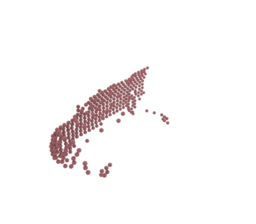
\includegraphics[width=2.25cm,trim={\cropleft cm \croplower cm \cropright cm \cropupper cm},clip]{gdat_shapenet_clean_low_165_points}
        \end{subfigure}
        \begin{subfigure}[t]{0.49\textwidth}
            \vspace{0px}\centering
            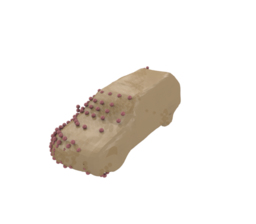
\includegraphics[width=2.25cm,trim={\cropleft cm \croplower cm \cropright cm \cropupper cm},clip]{gexp_clean_high_10_wide_vae_aml_3_2_res_165}
        \end{subfigure}
        \vspace*{-2px}
        \subcaption{ShapeNet (Synthetic)}
    \end{subfigure}
    \begin{subfigure}[t]{0.235\textwidth}
        \begin{subfigure}[t]{0.49\textwidth}
            \vspace{0px}\centering
            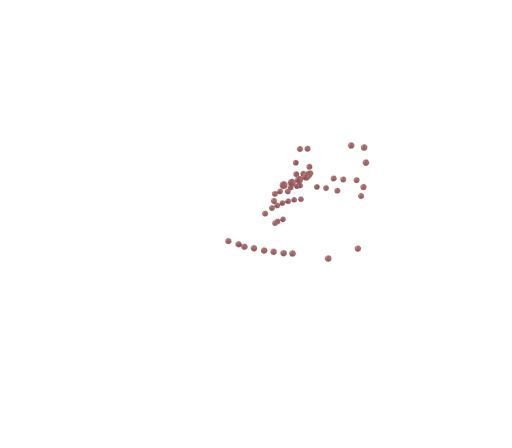
\includegraphics[width=2.25cm,trim={\cropleft cm \croplower cm \cropright cm \cropupper cm},clip]{gdat_kitti_1224_points}
        \end{subfigure}
        \begin{subfigure}[t]{0.49\textwidth}
            \vspace{0px}\centering
            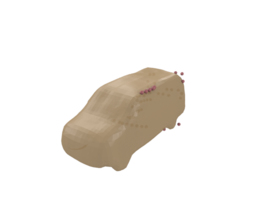
\includegraphics[width=2.25cm,trim={\cropleft cm \croplower cm \cropright cm \cropupper cm},clip]{gexp_cor_clean_medium_10_wide_w2_1_vae_aml_3_2_res_1224}
        \end{subfigure}
        \subcaption{KITTI (Real)}
    \end{subfigure}
    \\[2px]
    % 2233
    \begin{subfigure}[t]{0.235\textwidth}
        % 264 1188 1452
        \begin{subfigure}[t]{0.49\textwidth}
            \vspace{0px}\centering
            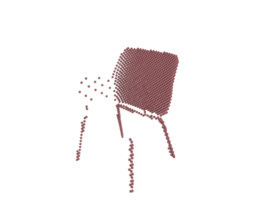
\includegraphics[width=2.25cm,trim={\cropleft cm \croplower cm \cropright cm \cropupper cm},clip]{gdat_modelnet_chair_high_1452_points}
        \end{subfigure}
        \begin{subfigure}[t]{0.49\textwidth}
            \vspace{0px}\centering
            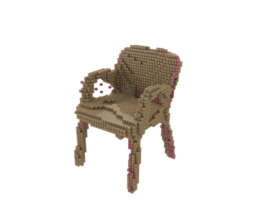
\includegraphics[width=2.25cm,trim={\cropleft cm \croplower cm \cropright cm \cropupper cm},clip]{gexp_clean_chair_high_10_wide_d_vae_aml_3_3_res_1452}
        \end{subfigure}
        \subcaption{ModelNet (Synthetic)}
    \end{subfigure}
    \begin{subfigure}[t]{0.235\textwidth}
        \begin{subfigure}[t]{0.49\textwidth}
            \vspace{0px}\centering
            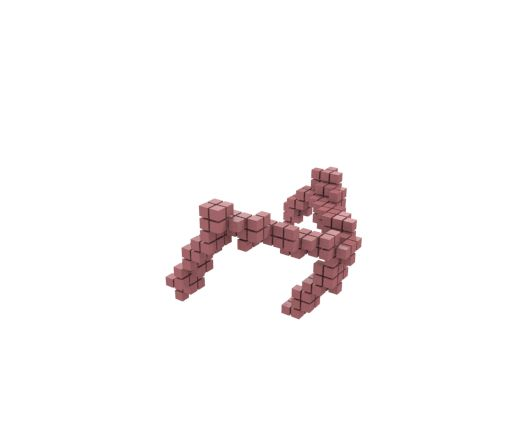
\includegraphics[width=2.25cm,trim={\cropleft cm \croplower cm \cropright cm \cropupper cm},clip]{gdat_yang_table_5_bin_points}
        \end{subfigure}
        \begin{subfigure}[t]{0.49\textwidth}
            \vspace{0px}\centering
            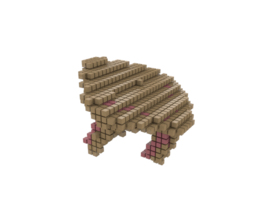
\includegraphics[width=2.25cm,trim={\cropleft cm \croplower cm \cropright cm \cropupper cm},clip]{gexp_clean_rtable_low_10_wide_vae_aml_3_3_res_5}
        \end{subfigure}
        \subcaption{\Kinect (Real)}
    \end{subfigure}
    }
    \vspace*{-\figskipcaption px}
    \caption{{\bf 3D Shape Completion.} Results for cars on ShapeNet \citep{Chang2015ARXIV} and KITTI \citep{Geiger2012CVPR} and for chairs and tables on ModelNet \citep{Wu2015CVPR} and \Kinect \citep{Yang2018ARXIVb}. Learning shape completion on real-world data is challenging due to sparse and noisy observations and missing ground truth. Occupancy grids (bottom) or meshes from signed distance functions (SDFs, top) at various resolutions in {\color{rbeige}beige} and point cloud observations in {\color{rred}red}.}
    \label{fig:introduction}
    \vspace*{-\figskipbelow px}
\end{figure}
\begin{figure*}
	\vspace*{-4px}
    \centering
    \begin{tikzpicture}
        % ---------------------------------------------------------
        \node[anchor=west] at (-1.25, 3.75) {{\footnotesize{\bf(1) Shape Prior} (Section 3.2)}};
        
        \node[rectangle,draw=black,anchor=west] (prior) at (-1,2.5) {
            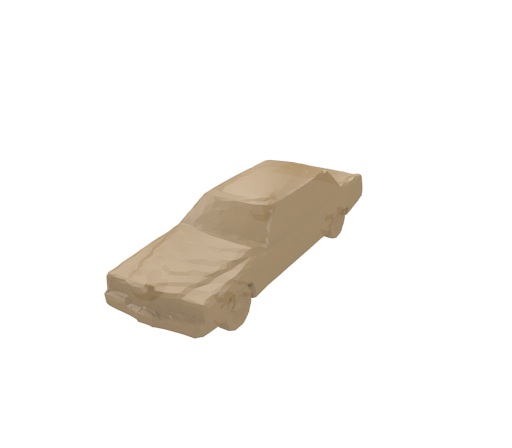
\includegraphics[height=1cm,trim={3cm 3cm 3cm 3cm},clip]{gfx_method_shapenet_66_gt_only}
            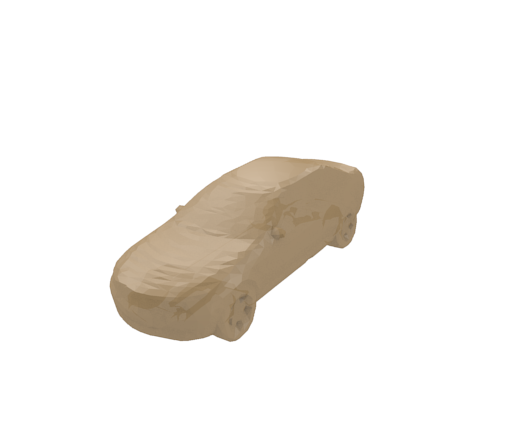
\includegraphics[height=1cm,trim={3cm 3cm 3cm 3cm},clip]{gfx_method_shapenet_132_gt_only}
            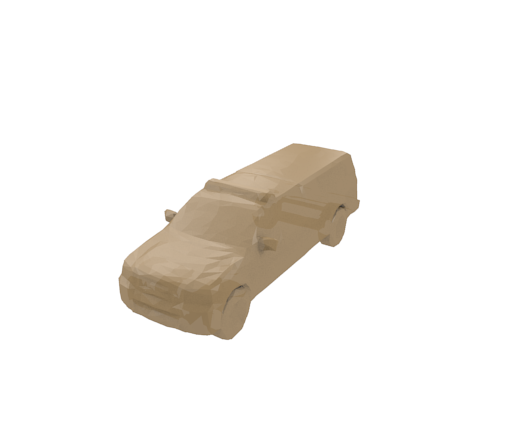
\includegraphics[height=1cm,trim={3cm 3cm 3cm 3cm},clip]{gfx_method_shapenet_198_gt_only}
            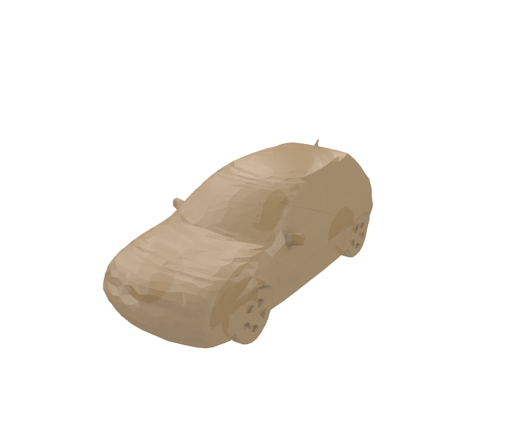
\includegraphics[height=1cm,trim={3cm 3cm 3cm 3cm},clip]{gfx_method_shapenet_264_gt_only}
        };
        \node at (1.6,3.3) {\scriptsize Synthetic Reference Shapes};
        
        \node[] (y) at (0, -1.5) {\scriptsize Shape $y$};
        
        \node[rectangle,draw=black,anchor=west] (input) at (-1, 0) {
            \begin{tabular}{c}
            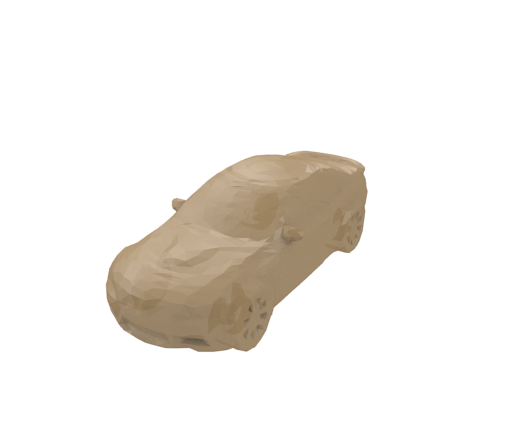
\includegraphics[height=1cm,trim={3cm 3cm 3cm 3cm},clip]{gfx_method_shapenet_0_gt_only}\\
            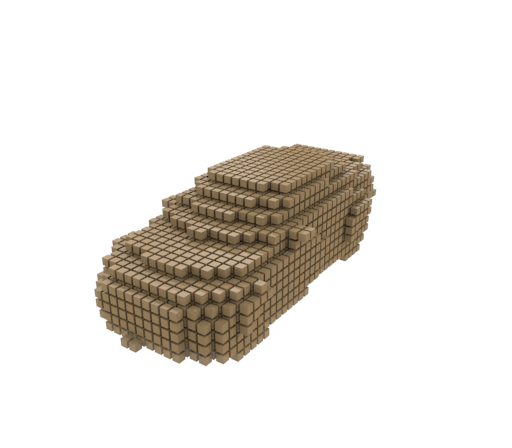
\includegraphics[height=1cm,trim={3cm 3cm 3cm 3cm},clip]{gfx_method_shapenet_0_bin_only}
            \end{tabular}
        };  
        
        \draw ($(input.north east) + (0.2,0)$) -- ($(input.north east) + (1.5,-0.75)$) -- ($(input.north east) + (1.5,-1.75)$) -- ($(input.south east) + (0.2,0)$) -- ($(input.north east) + (0.2,0)$);
        \node at ($(input.east) + (0.825,0)$) {\scriptsize encoder};
        
        \node (z) at (2.75, 0) {\scriptsize $z$};
        
        \node[rectangle,draw=black,anchor=east] (output) at (6.5, 0) {
            \begin{tabular}{c}
            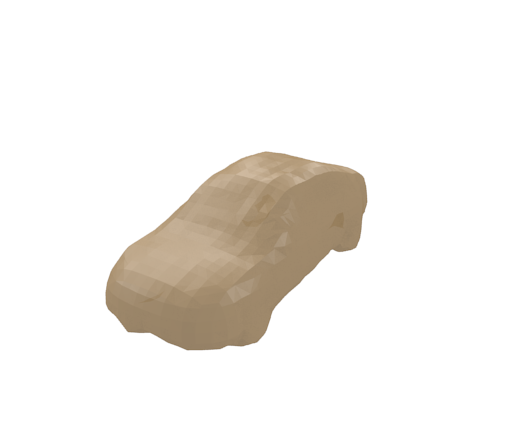
\includegraphics[height=1cm,trim={3cm 3cm 3cm 3cm},clip]{gfx_method_shapenet_3_2_res_0}\\
            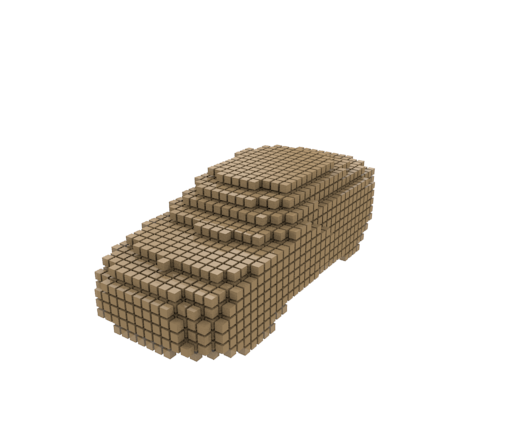
\includegraphics[height=1cm,trim={3cm 3cm 3cm 3cm},clip]{gfx_method_shapenet_3_3_results_only_results_0}
            \end{tabular}
        };
        
        \draw ($(output.north west) - (0.2,0)$) -- ($(output.north west) - (1.5,0.75)$) -- ($(output.north west) - (1.5,1.75)$) -- ($(output.south west) - (0.2,0)$) -- ($(output.north west) - (0.2,0)$);
        \node at ($(output.west) - (0.825,0)$) {\scriptsize decoder};
        
        \node (ry) at (5.5, -1.5) {\scriptsize Rec. Shape $\tilde{y}$};
        
        \node[] (L) at (2.75, -1.9) {\scriptsize Reconstruction Loss};
        
        \draw[-] (ry) -- ($(ry) - (0,0.4)$);
        \draw[-] ($(ry) - (0,0.4)$) -- (L);
        \draw[-] (y) -- ($(y) - (0,0.4)$);
        \draw[-] ($(y) - (0,0.4)$) -- (L);
        
        % --
        \draw[-] (3.5, 0.85) -- (3.5, 1.5);
        \draw[-] (3.5, 1.5) -- (12.5, 1.5);
        \draw[->] (12.5, 1.5) -- (12.5, 0.85);
        \node at (7.25, 1.75) {\scriptsize retain fixed decoder};
        
        \draw[-,dotted] (7.25,-2.15) -- (7.25,1.45);
        \draw[-,dotted] (7.25,2) -- (7.25,2.45);
        \draw[-,dotted] (7.25,3) -- (7.25,4.05);
        
        \node at (7.25, 2.75) {\scriptsize\textbf{no correspondence needed}};
        \begin{scope}[shift={(9,0)}]
        
        % ---------------------------------------------------------
        \node[anchor=west] at (-1.25, 3.75) {{\footnotesize{\bf(2) Shape Inference} (Section 3.3)}};
        
        \node[rectangle,draw=black,anchor=east] (inference) at (6.5,2.5) {
            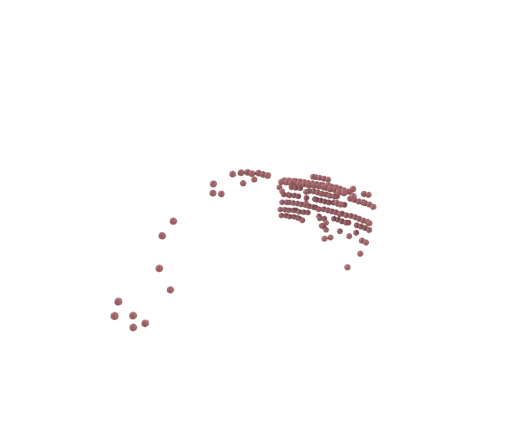
\includegraphics[height=1cm,trim={3cm 3cm 3cm 3cm},clip]{gfx_method_kitti_1530_points}
            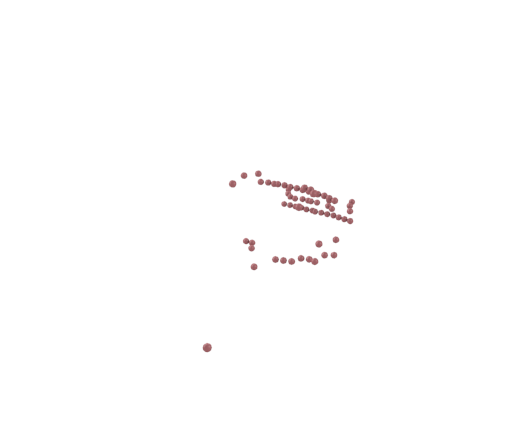
\includegraphics[height=1cm,trim={3cm 3cm 3cm 3cm},clip]{gfx_method_kitti_0_points}
            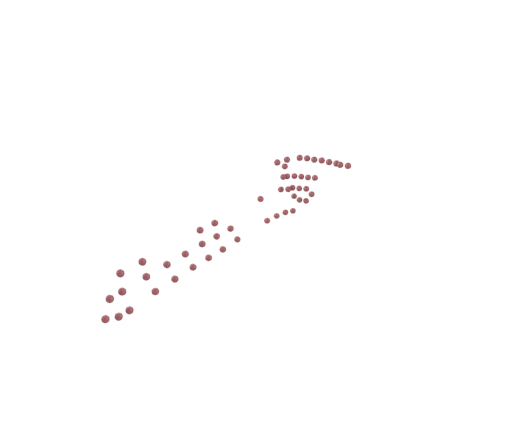
\includegraphics[height=1cm,trim={3cm 3cm 3cm 3cm},clip]{gfx_method_kitti_2448_points}
            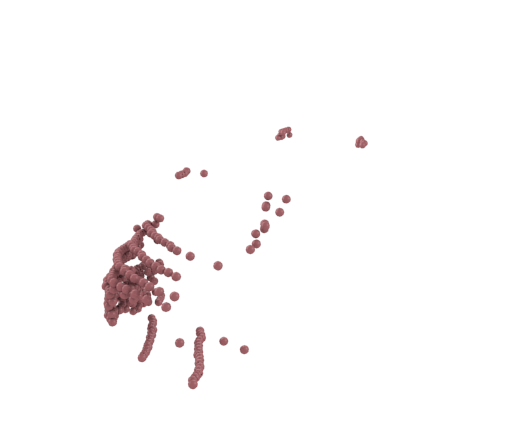
\includegraphics[height=1cm,trim={3cm 3cm 3cm 3cm},clip]{gfx_method_kitti_3366_points}
        };
        \node at (3.8,3.3) {\scriptsize Real Observations w/o Targets};
        
        % --
        \draw[-] (prior) -- (inference);
        
        \node[] (y) at (0, -1.5) {\scriptsize Observation $x$};
        
        \node[rectangle,draw=black,anchor=west] (input) at (-1, 0) {
            \begin{tabular}{c}
            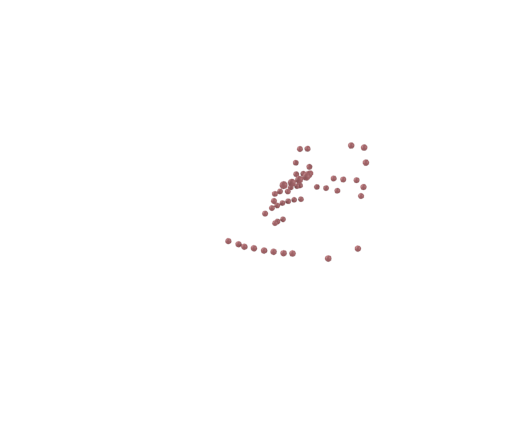
\includegraphics[height=1cm,trim={3cm 3cm 3cm 3cm},clip]{gfx_method_kitti_1224_points}\\
            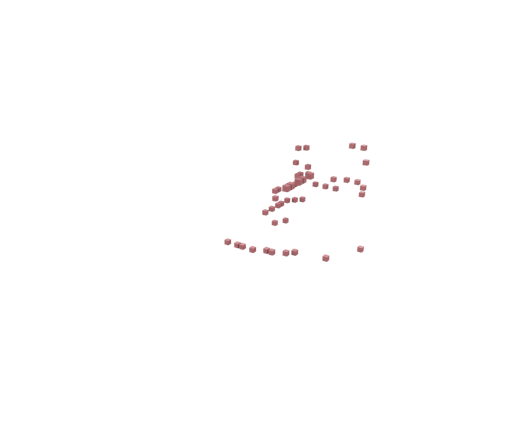
\includegraphics[height=1cm,trim={3cm 3cm 3cm 3cm},clip]{gfx_method_kitti_1224_bin_points}
            \end{tabular}
        };
        
        \draw ($(input.north east) + (0.2,0)$) -- ($(input.north east) + (1.5,-0.75)$) -- ($(input.north east) + (1.5,-1.75)$) -- ($(input.south east) + (0.2,0)$) -- ($(input.north east) + (0.2,0)$);
        \node at ($(input.east) + (0.825,0)$) {\scriptsize\begin{tabular}{c}new\\encoder\end{tabular}};
        
        \node (z) at (2.75, 0) {\scriptsize $z$};
        
        \node[rectangle,draw=black,anchor=east] (output) at (6.5, 0) {
            \begin{tabular}{c}
            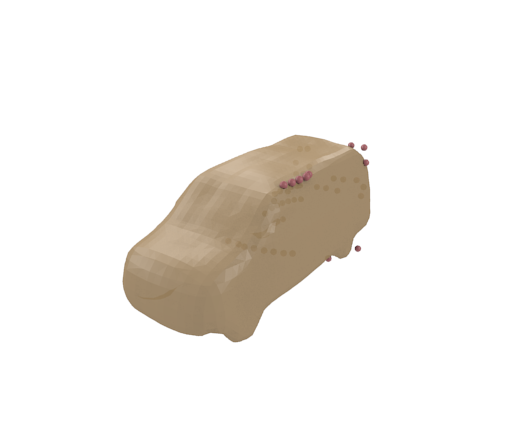
\includegraphics[height=1cm,trim={3cm 3cm 3cm 3cm},clip]{gfx_method_kitti_3_2_res_1224}\\
            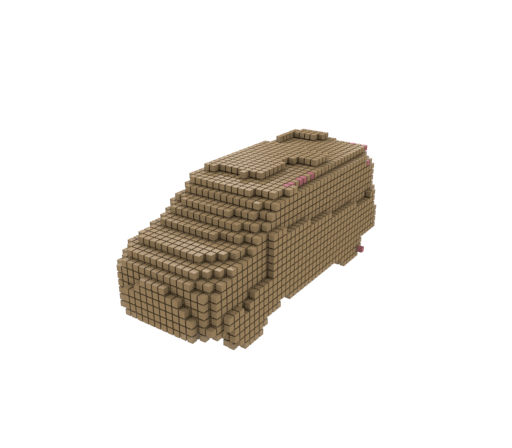
\includegraphics[height=1cm,trim={3cm 3cm 3cm 3cm},clip]{gfx_method_kitti_3_3_res_1224}
            \end{tabular}
        };
        
        \draw ($(output.north west) - (0.2,0)$) -- ($(output.north west) - (1.5,0.75)$) -- ($(output.north west) - (1.5,1.75)$) -- ($(output.south west) - (0.2,0)$) -- ($(output.north west) - (0.2,0)$);
        \node at ($(output.west) - (0.825,0)$) {\scriptsize \begin{tabular}{c}fixed\\decoder\end{tabular}};
        
        \node (ry) at (5.5, -1.5) {\scriptsize Prop. Shape $\tilde{y}$};
        
        \node[] (L) at (2.75, -1.9) {\scriptsize Maximum Likelihood Loss};
        
        \draw[-] (ry) -- ($(ry) - (0,0.4)$);
        \draw[-] ($(ry) - (0,0.4)$) -- (L);
        \draw[-] (y) -- ($(y) - (0,0.4)$);
        \draw[-] ($(y) - (0,0.4)$) -- (L);
        \end{scope}
    \end{tikzpicture}
    \vspace*{-12px}
    \caption{{{\bf Amortized Maximum Likelihood (AML) for 3D Shape Completion on KITTI.}
            (1) We train a denoising variational auto-encoder (\DVAE) \citep{Kingma2014ICLR,Im2017AAAI} as shape prior on ShapeNet using occupancy grids and signed distance functions (SDFs) to represent shapes. (2) The fixed generative model, \ie, decoder, then allows to learn shape completion using an unsupervised maximum likelihood (\ML) loss by training a new recognition model, \ie, encoder. The retained generative model constraints the space of possible shapes while the \ML loss aligns the predicted shape with the observations.}}
    \label{fig:method}
    \vspace*{-\figskipbelow px}
    \vspace*{\figskipbelow px}
\end{figure*}

3D shape perception is a long-standing and fundamental problem both in human and computer vision \citep{Pizlo2007CAIP,Pizlo2010,Furukawa2013FTCGV} with many applications to robotics. A large body of work focuses on 3D reconstruction, \eg, reconstructing objects or scenes from one or multiple views, which is an inherently ill-posed inverse problem where many configurations of shape, color, texture and lighting may result in the very same image. While the primary goal of human vision is to understand how the human visual system accomplishes such tasks, research in computer vision and robotics is focused on the task of devising 3D reconstruction systems. Generally, work by \cite{Pizlo2010} suggests that the constraints and priors used for 3D perception are innate and not learned. Similarly, in computer vision, cues and priors are commonly built into 3D reconstruction pipelines through explicit assumptions. Recently, however -- leveraging the success of deep learning -- researchers started to \emph{learn} shape models from large collections of data, as for example ShapeNet~\citep{Chang2015ARXIV}. Predominantly generative models have been used to learn how to generate, manipulate and reason about 3D shapes  \citep{Girdhar2016ECCV,Brock2016ARXIV,Sharma2016ARXIV,Wu2016NIPS,Wu2015CVPR}.

In this paper, we focus on the specific problem of inferring and completing 3D shapes based on sparse and  noisy 3D point observations as illustrated in \figref{fig:introduction}. This problem occurs when only a single view of an individual object is provided or large parts of the object are occluded as common in robotic applications. For example, autonomous vehicles are commonly equipped with LiDAR scanners providing a 360 degree point cloud of the surrounding environment in real-time. This point cloud is inherently incomplete: back and bottom of objects are typically occluded and -- depending on material properties -- the observations are sparse and noisy, see \figref{fig:introduction} (top-right) for an illustration. Similarly, indoor robots are generally equipped with low-cost, real-time RGB-D sensors providing noisy point clouds of the observed scene. In order to make informed decisions (\eg, for path planning and navigation), it is of utmost importance to efficiently establish a representation of the environment which is as complete as possible.

Existing approaches to 3D shape completion can be categorized into data-driven and learning-based methods. The former usually rely on learned shape priors and formulate shape completion as an optimization problem over the corresponding (lower-dimensional) latent space \citep{Rock2015CVPR,Haene2014CVPR,Li2015CGF,Engelmann2016GCPR,Nan2012TG,Bao2013CVPR,Dame2013CVPR,Ngyuen2016CVPR}. These approaches have demonstrated good performance on real data, \eg, on KITTI \citep{Geiger2012CVPR}, but are often slow in practice.

Learning-based approaches, in contrast, assume a fully supervised setting in order to directly learn shape completion on synthetic data \citep{Riegler2017THREEDV,Smith2017ARXIV,Dai2017CVPRa,Sharma2016ARXIV,Fan2017CVPR,Rezende2016ARXIV,Yang2018ARXIVb,Wang2017ICCV,Varley2017IROS,Han2017ICCV}. They offer advantages in terms of efficiency as prediction can be performed in a single forward pass, however, require full supervision during training. Unfortunately, even multiple, aggregated observations (\eg, from multiple views) will not be fully complete due to occlusion, sparse sampling of views and noise, see \figref{fig:results-real} (right column) for an example.

In this paper, we propose an amortized maximum likelihood approach for 3D shape completion (\cf \figref{fig:method}) avoiding the slow optimization problem of data-driven approaches and the required supervision of learning-based approaches. Specifically, we first learn a shape prior on synthetic shapes using a (denoising) variational auto-encoder \citep{Im2017AAAI,Kingma2014ICLR}. Subsequently, 3D shape completion can be formulated as a maximum likelihood problem. However, instead of maximizing the likelihood independently for distinct observations, we follow the idea of amortized inference \citep{Gersham2014COGSCI} and \emph{learn} to predict the maximum likelihood solutions directly. Towards this goal, we train a new encoder which embeds the observations in the same latent space using an unsupervised maximum likelihood loss. This allows us to learn 3D shape completion in challenging real-world situations, \eg, on KITTI, and obtain sub-voxel accurate results using signed distance functions at resolutions up to $64^3$ voxels. For experimental evaluation, we introduce two novel, synthetic shape completion benchmarks based on ShapeNet and ModelNet \citep{Wu2015CVPR}. We compare our approach to the data-driven approach by \cite{Engelmann2016GCPR}, a baseline inspired by \cite{Gupta2015CVPR} and the fully-supervised learning-based approach by \cite{Dai2017CVPRa}; we additionally present experiments on real data from KITTI and \Kinect \citep{Yang2018ARXIVb}. Experiments show that our approach outperforms data-driven techniques and rivals learning-based techniques while significantly reducing inference time and using only a fraction of supervision.

A preliminary version of this work has been published at CVPR'18 \citep{Stutz2018CVPR}. However, we improved the proposed shape completion method, the constructed datasets and present more extensive experiments. In particular, we extended our weakly-supervised amortized maximum likelihood approach to enforce more variety and increase visual quality significantly. On ShapeNet and ModelNet, we use volumetric fusion to obtain more detailed, watertight meshes and manually selected -- per object-category -- $220$ high-quality models to synthesize challenging observations. We additionally increased the spatial resolution and consider two additional baselines \citep{Dai2017CVPRa,Gupta2015CVPR}. Our code and datasets will be made publicly available\footnote{\url{https://avg.is.tuebingen.mpg.de/research_projects/3d-shape-completion}.}.

The paper is structured as follows: We discuss related work in \secref{sec:related-work}. In \secref{sec:method} we introduce the weakly-supervised shape completion problem and describe the proposed amortized maximum likelihood approach. Subsequently, we introduce our synthetic shape completion benchmarks and discuss the data preparation for KITTI and \Kinect in \secref{sec:data}. Next, we discuss evaluation in \secref{sec:evaluation}, our training procedure in \secref{sec:training}, and the evaluated baselines in \secref{sec:baselines}. Finally, we present experimental results in \secref{sec:experiments} and conclude in \secref{sec:conclusion}.